\chapter{Literature Review}
	\setcounter{secnumdepth}{2}
		\section{Cycle Analysis and Propulsion System Design Requirements}
		As discussed previously, the typical tool set for the engine designer at the conceptual level is engine thermodynamic cycle analysis.  The point of the cycle analysis at the conceptual level is to establish an engine aerothermodynamic cycle which can satisfy all of the requirements of the engine while minimizing operational costs such as fuel burn.  In the early years of cycle analysis, cycle trade studies were the primary tools for conducting the parametric engine cycle design studies, while the advent of the modern computer and computer aided design has enabled the integration of other aspects of the design process such as engine flowpath, aircraft mission and cost analyses.  Additionally, modern design techniques enable broad trade space exploration and optimization within the context of these computational models.  Along the same lines, engine and airframe integration, especially in the military realm, has had a similar history with increasing tendency towards integrated design processes to facilitate increasing design knowledge early in the design phase to eliminate costly design changes in the later phases.  This section will look at the latest cycle analysis techniques and the basics of sub-sonic inlet integration.
		
		\subsection{The Subsonic Airframe Integration Process}
		\indent Since this thesis primarily will focus on BLI for reduction in civil aviation fuel burn, it is worth looking at the current inlet and engine integration processes and requirements which are typical and to also consider how the BLI concept might change this paradigm.  Firstly, civil transports of the kind to be considered for BLI will spend the vast majority of their time at the cruise condition.  For that reason, cruise fuel burn is typically considered the metric of interest in most studies.  However, of course it is worth mentioning that cruise does not take place at a fixed altitude, but rather a range of altitudes and Mach numbers during flight, with the vehicle lift, angle of attack, and pressure distribution changing as fuel is burned.  Typically the engine is sized for some value of thrust at the top-of-climb condition where mass flow is a maximum.  Additionally, there is typically some maximum specified turbine inlet temperature at take-off where the engine is running at its hottest, and the engine has to be able to supply the necessary thrust to achieve a particular take-off field length and climb rate.  The point is that there are a large range of operating conditions from take-off through climb, cruise, and descent which the inlet must supply sufficiently clean air for the propulsion system to supply the necessary thrust power to fly the vehicle.  At each of these flight conditions, there is a different interaction between the airframe boundary layer and the engine than at the cruise condition.  This difference will have an impact on performance through the BLI effects discussed in previous sections, but also on the ability of the propulsion system to meet the requirements.  Uncertainty in these interactions could lead to mistakes in design choices or fundamentally overestimated benefit of the technology, leading to a totally inferior aircraft relative to the state of the art podded engines.  Such mistakes could have catastrophic consequences considering the modern economic climate.
		
		\subsubsection{Subsonic Flow Incidence Requirements}
		\indent Although the inlet and airframe integration process is somewhat less tedious than for the military case, since civil transports clearly do not have as many critical maneuvers as military planes, the point still remains that there are multiple conditions in which the geometric orientation of the airframe causes potential problems for an engine inlet.  Perhaps most important among these are conditions such as take-off, climb, and landing where the vehicle and engine might be at an increased angle of incidence relative to the free-stream.  The inlet mass flow ratio is the parameter that best describes the approaching flow and is given by equation \ref{Mass_Flow_Ratio}.
		\begin{equation}
			\frac{A_o}{A_i} = \frac{\Big(\dot{m}_2 \sqrt{\theta_2}/\delta_2\Big)\Big(\delta_2/\delta_o\Big)}{\Big(\dot{m}\sqrt{\theta}/\delta A\Big)_o\Big(A_i\Big)} = \frac{\Big(\dot{m}\sqrt{\theta}/\delta\Big)_2\Big(\pi_d\Big)}{\Big(\dot{m}\sqrt{\theta}/\delta A\Big)_o\Big(A_i\Big)}
			{}
			\label{Mass_Flow_Ratio}
		\end{equation}%
		\indent Oates states that:  "For subsonic inlets, the numerical value of $A_o/A_i$ is a direct indication of the general incidence of the flow approaching the inlet.  A value of unity means that the inlet is capturing its projection in the freestream and the stagnation point will occur at the inlet highlight for level flight.  A value less than unity indicates flow is prediffusing in the freestream, such that an outward flow incidence occurs; this is generally the case for cruise flight speeds.  Conversely,$A_o/A_i$ will exceed unity at low flight speeds and moderate to high power settings, such that an inward flow incidence develops with the stagnation point on the outer portion of the lip."  Furthermore, other flight conditions in which flow incidence is induced produce a velocity component normal to the freestream on top of the basic mass flow effect.   Figure \ref{Inlet_Incidence_Schematic} illustrates these issues \cite{Oates1989} for different flight conditions.
		%%
		\begin{figure}[htpb]
			\centering
			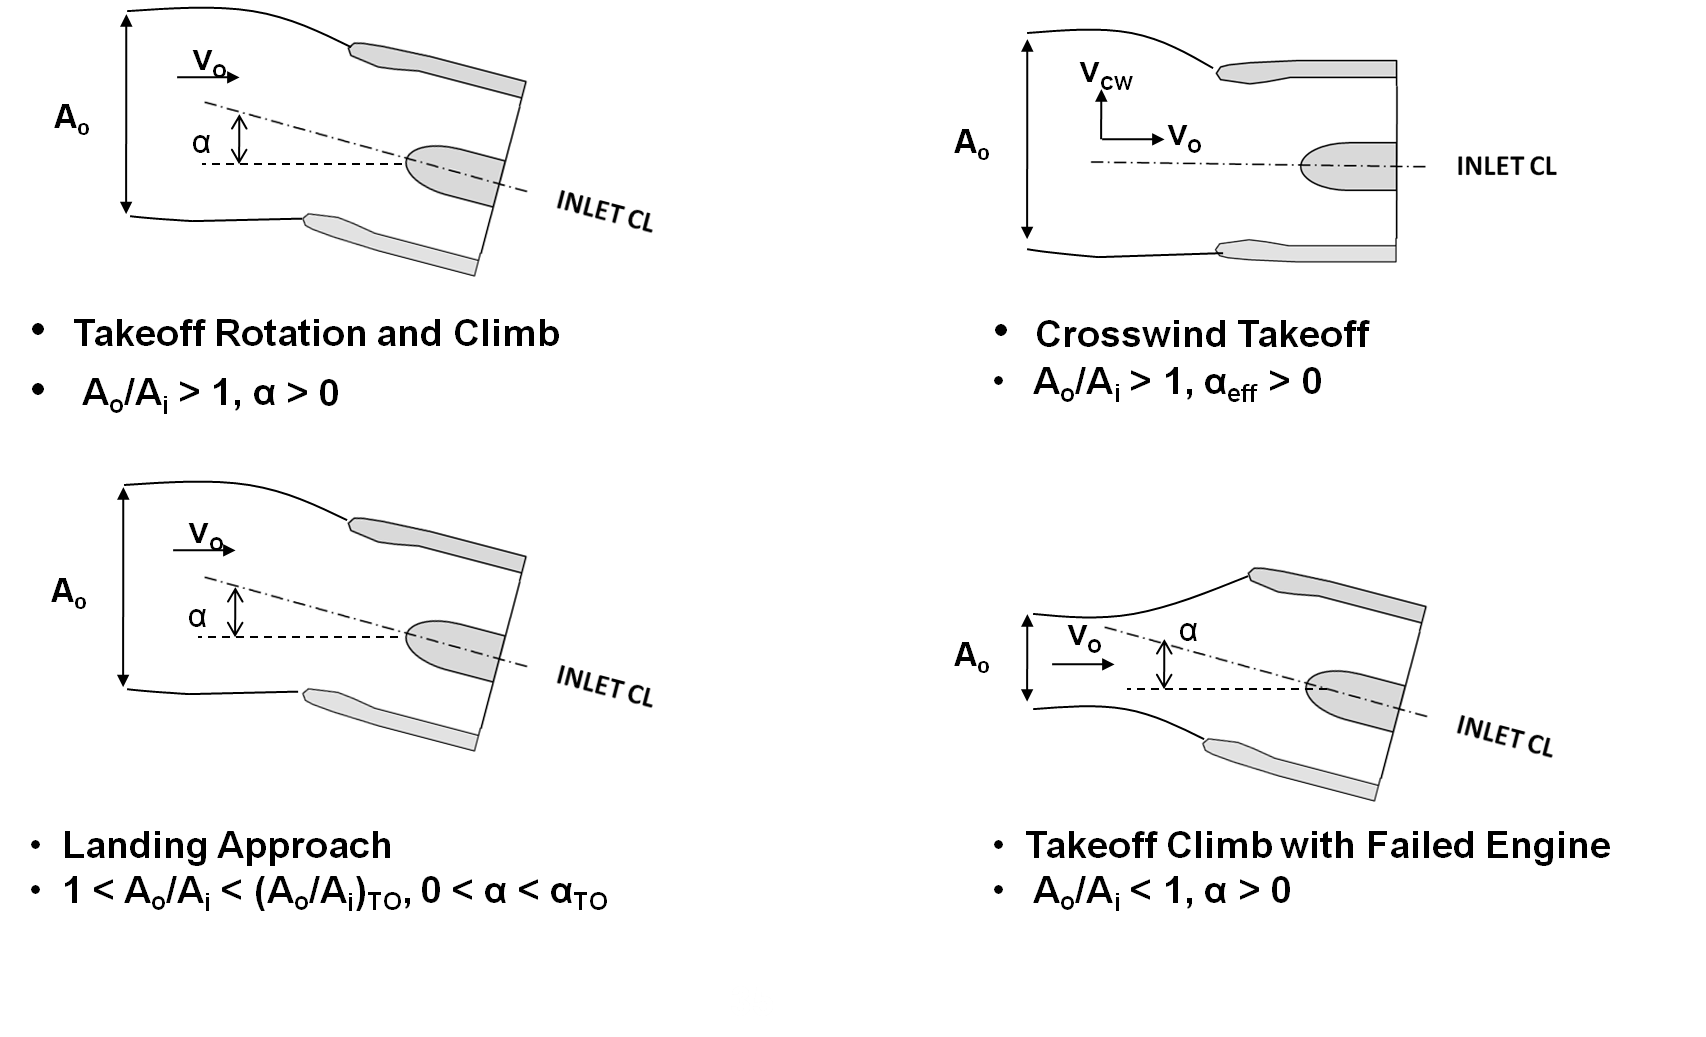
\includegraphics[width=140mm, height =85mm, clip=true, trim = 0mm 0mm 0mm 0mm]{Inlet_Incidence_Conditions.png}
			\caption{Notional inlet diagrams showing different conditions for which there are high inlet incidence angles \cite{Oates1989}}
			\label{Circumferential_Distortion}
		\end{figure}
		%%
		For each of these flight conditions, there is a danger that the flow could separate as it passes over the lower inlet lip, thus producing potentially unacceptable distortion levels.  The engine must still be able to supply relatively low distortion flow to the inlet such that the engine maintains thrust and does not surge.  Furthermore, this condition must be satisfied over a range of free-stream Mach numbers, since the aircraft is accelerating during climb and deccelerating during landing.  Typical engine incidence requirements are shown plotted vs. freestream Mach number in figure \ref{Alpha_Incidence_Requirements}.  
		
		%%
		\begin{figure}[htpb]
			\centering
			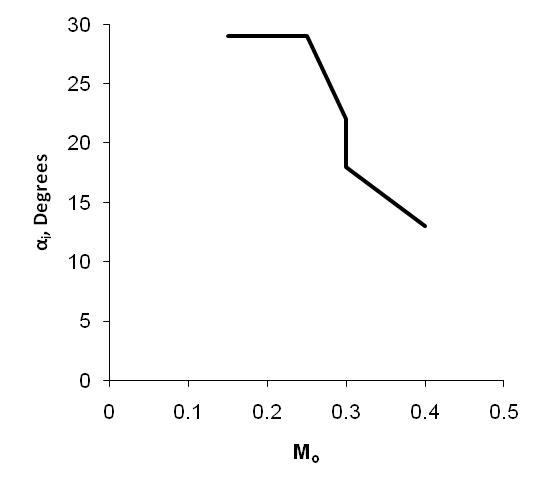
\includegraphics[width=120mm, height =85mm, clip=true, trim = 0mm 0mm 0mm 0mm]{Alpha_Incidence_Requirements.png}
			\caption{Notional inlet incidence angle requirements vs. freestream Mach number \cite{Oates1989}}
			\label{Alpha_Incidence_Requirements}
		\end{figure}
		%%
		
		Finally, it is worth discussing the take-off with engine out condition.  This is critical since the engine is operating at peak temperature during take-off meaning that a failure is likely to happen at that condition since the majority of the damage to the components occurs there.  If an engine goes out, the ingested mass flow ratio is significantly less than unity since the engine is windmilling.  At this condition, the external cowl can produce significant drag due to the flow accelerating rapidly over the cowl lip.  The remaining operating engines must be able to overcome this drag on it's own with sufficient climb rate.  
		
		\subsection{BLI as a Paradigm Shift}
		\indent With the preceeding understanding of the limiting flight conditions for typical subsonic inlet integration, it is now necessary to consider how the above might change if there is some base level of distortion being ingested into the engine.  Firstly, the fundamental difference between the embedded engine and the podded engine is that the danger due to separation is coming from the airframe itself rather than the inlet lip.  This means that the level of distortion is inherently greater and the consequence of flow separation potentially greater as well.  It is logical to speculate then, that the BLI engines will struggle to meet the vehicle incidence requirements.  Indeed, the angle of attack envelope of the vehicle may need to be limited by the distortion limits of the engine as a function of Mach number.  All of this has hitherto been unaddressed in the analysis literature, even with computational fluids tools, much less in the system study literature.  Since these concerns may ultimately limit the possible engine configurations and also impact the cycle designs, there is a need to integrate these design conditions into conceptual design cycle analysis framework to at minimum understand their impact.  
		
		\indent Another level of complexity generated by the boundary layer ingesting engine has to do with the placement of the engines on the airframe.  First, the placement of each engine (or array of engines in the case of distributed propulsion) is now a design variable, although it is certainly subject to key constraints such as stability and control and similar practical concerns.  Furthermore, since preceeding sections have substantiated that having smaller engines distributed across the airframe suction surface potentially offers higher BLI propulsive efficiency gains, there is a problem of having different airframe-engine interference for different sets of engines.  For instance, if there are three engines such as in the work of Rodriguez \cite{RodriguezThesis}, then the centerline engine may have quite different inlet flow properties -- primarily boundary layer thickness -- and subsequent performance impacts.  As a corollary to this, Rodriguez showed that a proper inlet aerodynamic optimization might yield different inlet designs and slighty different inlet orientation for the inboard and outboard.  This would then mean that the recoveries and distortion levels between the engines are different even though each engine is subject to the same operability constraints.  To date, one system study has looked at the possibility of quantifying the impact of this \cite{Sato2011} effect in terms of the BLI propulsive efficiency benefit.  This study determined that if one does not consider the effect in the fuel burn calculations, then BLI benefit is rather significantly over predicted (which for BLI could mean 1 or 2\%).  Another computational fluids study \cite{Kim2012} which showed this effect was done for the Boeing N2B design, in which the boundary layer thickness was found to differ by as much as a factor or two between inboard and outboard propulsors.
		
		\subsection{BLI Cycle Analysis Approaches}
		\indent To date, the cycle analysis requirements specified in the BLI engine design literature have been of the traditional style.  Typically a sizing point is set, such as top-of-climb, and the engine size is based on the required mass flow to achieve the engine thrust at that point.  A few authors have additionally included analyses of the off-design points to check for sufficient sea-level static and take-off thrusts \cite{Felder2011} \cite{Sato2011}.  Most of the higher fidelity studies do not touch the engine models, with perhaps the exception of Rodriguez who did vary the engine bypass ratio independently and used the cruise point as the engine sizing point \cite{RodriguezThesis} \cite{Rodriguez2009}.			
		%%Put method of Pratt and Whitney in this
		
	\section{Boundary Layer Ingestion Models}
	
		There are various approaches for modeling the effect of boundary layer ingestion on an aircraft.  The primary differences between these methods is the fidelity of the models and the design capabilities that they allow.  Some of the simpler models have basic, conceptual level parameters which define inputs to the model and with which the designer can understand the relevant trends.  Higher order methods tend to be less parametric and require much more computational time, and for that reason are typically reserved for the later stages of design where detailed design features need to be set, and the uncertainty in the result must be inherently lower.  Since this thesis work focuses on engine design at the very earliest conceptual stages in the context of BLI, the focus of this chapter is to outline some of the major approaches that have been taken to model BLI at the conceptual level.  The purpose of this chapter is to outline the basic theory of each of these models, summarize the results from previous studies which employed them, and to assess the relative short-comings and benefits of each of them to provide a basis for later model selection and adaptation.  Additionally, this chapter will substantiate the need for the current work by outlining the overall shortcomings of previous approaches to identify areas of improvement in both modeling and design methodology.

	\section{Boundary Layer Ingestion Literature Review}
		\subsection{Classic Studies}
			Boundary layer ingestion really stems from considerable usage in marine propulsion where it is much easier to take advantage of the large ship wake that can be ingested by an aft mounted propeller.  It has been researched somewhat in previous investigations for aircraft applications however.  The first investigation of BLI was conducted by A.M.O. Smith \cite{Smith1947}.  In 1946, Smith conducted an analysis of a turbojet engine and aircraft design with standard inlets and with BLI inlets. The BLI inlets were idealized as slots installed over the wing.  Smith showed a 30\% improvement in fuel efficiency and a 7\% higher optimum cruise speed, though this is in comparison to designs of the time.
	
			Lynch \cite{Lynch1960} performed a momentum analysis on an early turbofan engine design that ingested fuselage boundary layer and obtained a 3\% improvement in propulsive efficiency accompanied by a 6-10\% decrease in maximum engine thrust. Lynch’s analysis also depended on the assumption of minimal inlet losses.
			
			Douglass \cite{Douglass1970} performed an energy wake analysis on an aircraft with aft fuselage-mounted engines. The engines were assumed close enough to the fuselage to ingest the boundary layer. Douglass’ analysis suggests up to a 10\% improvement in propulsive efficiency compared to an equivalent pylon mounted engine installation. 

		\subsection{Recent System Studies}
			There has been a significant amount of research conducted on the BLI concept in essentially the last decade.  This work has focused on many different vehicle concepts as well as many different aspects of the problem ranging from system level trade studies and technology risk assessment to high-order computational analyses and optimization of inlets and nacelles.  There have also been some funded experimental studies, leaving at least a small amount of experimental data for certain designs -- most commonly the inlet and fan.  This thesis pertains to system studies at the conceptual level and so the following section will summarize in some detail the goals, general modeling approach, and conclusions of recent system level studies as well as show a comparison of the high level benefit for each of the identified studies.  

			\subsubsection{Boeing Studies}
				Dagget et. al. conducted a study for the Boeing company under the Ultra Efficient Engine Technology/Propulsion Airframe Integration Project.  The study was designed to analyze the effect of BLI on the BWB aircraft with active flow control (AFC).  The engine analysis was done using the "ram drag" approach, meaning that the ram drag term contained within the net thrust is reduced by a percentage which is calculated based upon the boundary layer characteristic averaged over its height.  The analysis included 3 tasks:  first the establishment of a baseline; second, the evaluation of embedded engines with BLI; third, evaluation of active flow control (AFC) to inlets.  A podded engine based off of typical engine technology was established as the baseline engine.  For the BLI configuration, a long S-Duct, highly off-set embedded inlet was used to establish the fuel burn benefits from the ram drag reduction.  It was determined that the baseline BLI configuration would offer 3.1\% fuel burn improvement, which is relatively substantial.  With the addition of the AFC technology, the inlet duct can be shortened which has weight, wetted area, and total engine length benefits.  This also allows the use of high aspect ratio inlets which allows for larger ingested boundary layer.  The fuel burn benefit with the AFC technology and the shorter low-offset inlets was estimated as 5.5\%.  
				
				\indent Another study conducted by the Boeing company focused on the inlet configuration and the potential benefits offered by increasing the aspect ratio of the inlet.  The approach and general vehicle configuration was very similar to that studied in ref. XX.  The study also refined the calculation for the nacelle viscous drag by "proper analyses of viscous changes where reductions in nacelle drag account for local Reynolds Number effects".  This accounting difference led to a much greater estimate of the potential of BLI with AFC and flush mounted inlets which was estimated at ~10\% maximum.  It was determined that the lower aspect ratio inlet (higher height than width) resulted in a better net fuel burn than the larger width inlets due to the fact that the inlet pressure recovery was assumed to be 1\% different.  The result of this is therefore dependent on the validity of this assumption.  If the lower and wider inlet (higher AR) can be kept at sufficiently similar levels of inlet recovery, it should offer larger benefit due to the increased amount of drag ingestion and improved ram drag effect.

			\subsubsection{Nickols}
				\indent Nickols and McCullers conducted a configuration system study for the Hybrid Wing Body concept.  This study was a relatively low fidelity study which did not truly employ engine design techniques or cycle analysis.  Instead the study assumed a certain percentage drag reduction to be applied to the aircraft drag polar within the mission analysis, as well as a nacelle wetted area reduction factor, pylon weight sturctural factor, and SFC penalty due to the lower inlet pressure recovery.  The final analysis showed an impact of 5.2\% fuel burn benefit for the BLI technology.

			\subsubsection{Rodriguez}
				\indent Rodriguez, as a part of his doctoral work, developed a method for multi-disciplinary inlet optimization which combined high fidelity CFD methods with a propulsion model.  The method was applied to the BWB vehicle with 3 boundary layer ingesting high-bypass ratio engines.  The method consisted of optimizing the inlet and external cowl shape such that the fuel burn rate is minimized while maintaining an acceptable level of inlet distortion.  The method itself did show significant improvement from the baseline design, which highlights the importance of higher-order methods in the detail aerodynamic design phase.  However, the work showed that the same optimization applied to the podded case yielded the result that BLI did not provide any benefit (BLI was actually worse, in fact).  This could have resulted from the fact that there were a limited number of design variables for the outboard engines, yielding excess and potentially removable wave drag from the outboard engines.  Furthermore, the inlet pressure recovery was very low in comparison to recent studies which have shown potentially much higher values of inlet recovery using other optimization methods.

			\subsubsection{Plas}
				\indent As part of NASA's silent aircraft initiative, Plas conducted a study of boundary layer ingesting engines in which the following 3 contributions were intended:  Creation of a conceptual and theoretical framework for BLI in aircraft design; development of high fidelity models for representing an aircraft with BLI embedded engines; Quantification of the benefits of BLI.  This work is the first of it's kind that actually analyzes the impacts of BLI while including an actual model of the turbomachinery operating in non-uniform flow.  The study assumed that the configuration of interest was a ducted fan type.  The work included an assessment of three different degrees of fidelity within the fan modeling:  a one-dimensional parallel compressor approach, an integral boundary layer approach, and a 3-D body force model.  The highest fidelity of these approaches showed that BLI for the aircraft under consideration in the silent aircraft initiative gave power savings between 3-4\%.  The study also concluded that a principal feature required to estimate power saving for the propulsor is the distortion transfer across the fan (i.e. level of distortion downstream of the fan).  It was also found that the power savings differed by 10-40\% between the different fidelity fan models, although the trends remained roughly the same regardless of the modeling fidelity.

			\subsubsection{NASA and UTRC}
				\indent Hardin et. al conducted an aircraft system study of a BLI propulsion configuration.  The analysis included a detailed cycle model for an ultra-high-bypass propulsion system with BLI.  The system study employed lower order models for the different components of the BLI problem, including the BLI theoretical benefits; nacelle weight and drag; fan performance; and inlet pressure losses.  Aircraft trade factors were used to estimate fuel burn based on the engine cycle calculations and weight estimates, and the results of the study showed that a 3-5\% BLI fuel burn benefit could be achieved for the "N+2" generation aircraft relative to a pylon mounted baseline.  Another key conclusion was that the inlet pressure recovery and fan efficiency have a strong impact on the level of fuel burn achieved with 1\% pressure recovery loss translating to 3\% fuel burn increase.  This provides the motivation for low loss inlets and distortion tolerant fan configurations to maximize the potential benefit of the technology.

			\subsubsection{Summary}
				\indent A few trends arise from an analysis of the system study literature:

				\begin{figure}[hptb]
					\centering
					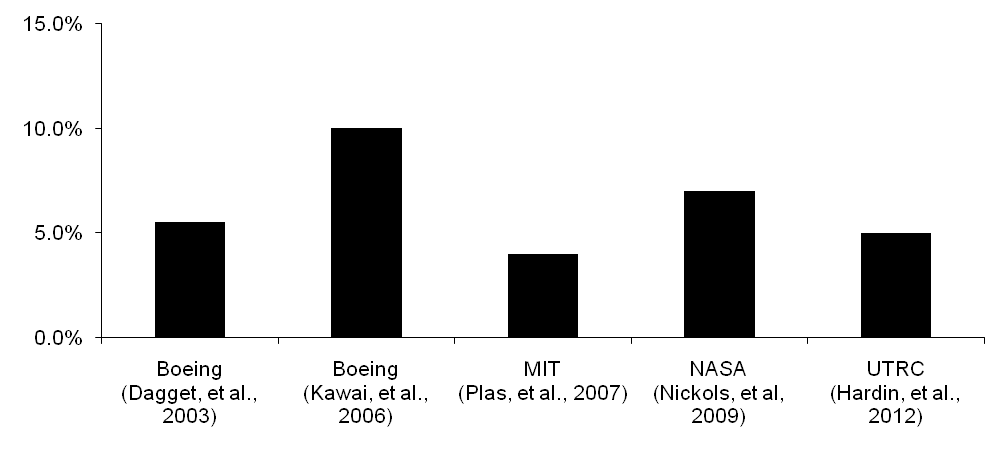
\includegraphics[width=120mm, height =60mm]{Figure4_System_Study_Estimates.png}
					\caption{Boundary layer ingestion system study estimates}
					\label{System_Estimates}
				\end{figure}
				
				\begin{itemize}
				\item{The fuel burn analysis for BLI is a function of the trade-offs between propulsive efficiency gains obtained via drag ingestion, thermal efficiency penalty due to distorted inlet flow, propulsive efficiency changes due to changes in nacelle and interference drag, and the effect on the engine and support structure weight -- all of which affect the aircraft fuel burn.}
				\item{There is a wide uncertainty on the potential benefit that BLI offers for the HWB aircraft, typically ranging from 0-10\%. (See fig. \ref{System_Estimates})}
				\item{The quality of the inlet, level of inlet distortion, and impact on the fan efficiency have a strong impact on the potential benefits.  This is shown by simple cycle analysis results, as well as by the study of Rodriguez, which predicted no benefit for BLI with very high loss inlets relative to studies with much improved assumptions.}
				\item{Configurations which can reasonably ingest more boundary layer across the upper surface of the aircraft stand to offer larger potential benefits.}
				\end{itemize}

	\section{Modeling Requirements for BLI}
		The boundary layer ingestion problem can be broken down into two areas with regard to performance:  propulsive efficiency improvement (BLI effect) and thermal efficiency degradation.  This is the basic trade-off upon which the economic viability of the system depends.  This is an almost trivial statement, since of course the overall efficiency of the engine is ultimately a product of the thermal and propulsive efficiencies.  However, the thing that makes the BLI problem interesting at the conceptual level is that the negative (thermal) efficiency impacts and the positive (propulsive) efficiency impacts are both functions of how much boundary layer (distorted flow) enters the engines.  As more drag is ingested into the engine, the propulsive efficiency benefits increase, however the level of distortion and general total pressure recovery decreases which impacts the performance of the propulsor and potentially the gas turbine core.  The design challenge then, stated clearly, is to maximize the amount of drag ingested while maintaining sufficiently low levels of distortion and total pressure loss such that the benefits of the propulsive efficiency gain are not prohibitive.  
		\begin{figure}[htpb]
			\centering
			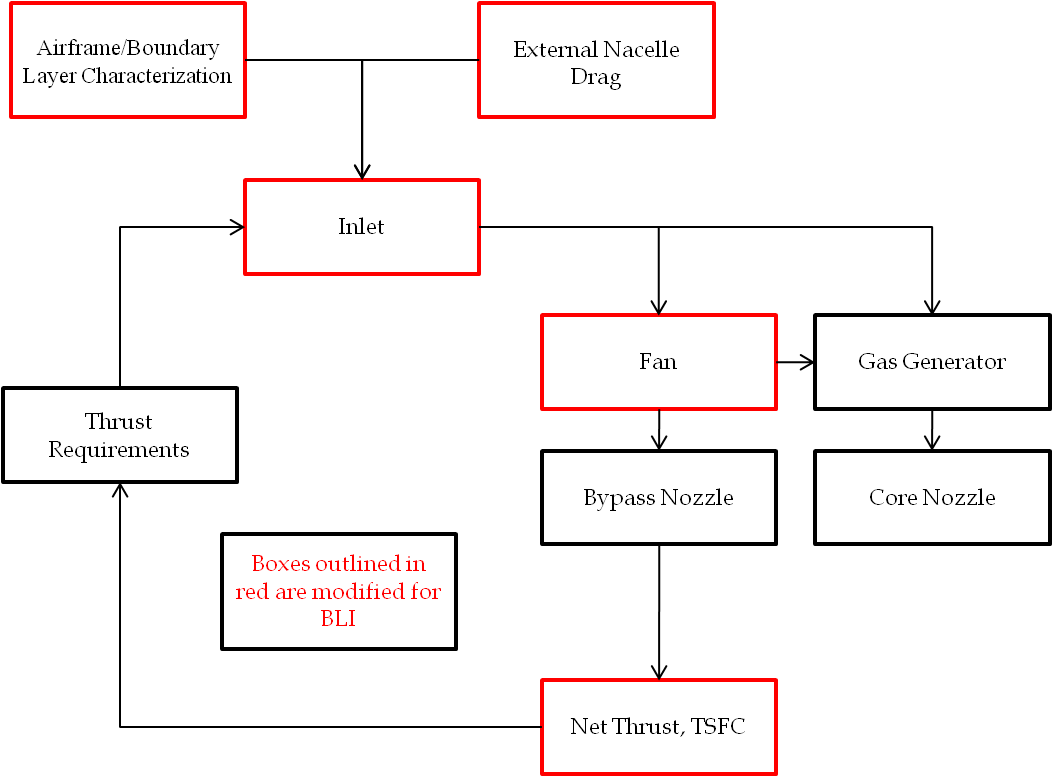
\includegraphics[width=140mm, height =80mm, trim=0mm 0mm 0mm 0mm, clip=true]{Figure2_Cycle_Analysis_with_BLI.png}
			\caption{Notional cycle analysis for a BLI propulsion system.  Boxes outlined in red show the components which need modification for BLI.}
			\label{BLI_changes}
		\end{figure}
		To do this, the designer must have proper modeling fidelity for each of the components which are impacted by the ingestion.  Design trades would then emerge from the combination of the various impacts on each component via typical cycle analysis techniques.  Fig. \ref{BLI_changes} shows the components which require modification or addition for BLI.  These are the most basic components that require modeling, however there can be other effects which impact system performance.  These include but are not limited to: impact on bypass nozzle gross thrust coefficient; impact on propulsion system weight relative to equivalent podded case; compression system stability (fan or core stall).
		The rest of the chapter will focus on describing the state of the art system level approaches taken for each of the above components which require BLI impact modeling.  Some space will also be taken to describe cycle analysis methodology.   
	
	\section{Airframe Aerodynamics and Boundary Layer}
		The previous section discussed the power balance method and the metrics by which BLI performance can be estimated.  These turned out to be a function of the characteristics of the aerodynamics of the vehicle and specifically the boundary layer properties such as the momentum and kinetic energy thicknesses as well as the shape factors.  This section will discuss the methods by which system studies have estimated the inviscid airframe properties as well as the boundary layer properties needed for the performance analysis.

		\subsection{Boundary Layer Characterization}
			\indent There are a few general methods used to generate the airframe boundary layers.  The two primary methods for conceptual level system studies are summarized in Table \ref{Methods_Airframe}.  
			\begin{table}[htp]
				\centering
				\begin{tabular}{| >{\centering}m{4.5cm} | >{\centering}m{4.5cm} | m{4.5cm} |} 
					\hline
					Approach & Pros & Cons 
					\\
					\hline 
						1-D Boundary Layer Profiles 
					&   
						\begin{itemize}
							\item{Simple}
							\item{Fast}
							\item{Closed form solution}
							\item{Scalable with Reynolds}
						\end{itemize} 
					& 
						\begin{itemize}
							\item{Can't capture 2-D/airframe effects}
							\item{No angle of attack variation}
						\end{itemize} 
					\\
					\hline
						CFD Based Boundary Layer Profiles 
					& 
						\begin{itemize}
							\item{Captures Airframe Effects}
						\end{itemize} 
					&
						\begin{itemize}
							\item{Not scalable}
							\item{Data only at points where CFD is run}	
							\item{Expensive/time consuming}																							
						\end{itemize} 	
					\\																			
					\hline
				\end{tabular}
				\caption{Summary of the two prominent methods for boundary layer characterization and their pros and cons for system level conceptual design studies with BLI.}
				\label{Methods_Airframe}
			\end{table}  		
			Studies which use the first method include \cite{Sato2011} \cite{Plas2007}, and studies which use the second type of method include  \cite{Felder2011} \cite{Hardin2012} \cite{Kawai2006}.  The majority of system level studies avoid using CFD in the multi-disciplinary analysis loop, but rather assume that the boundary layers do not change much from the cruise point and simply use those profiles as a starting point.  From the first method, typical approaches are to assume a Coles wake profile or a $1/7^{th}$ power law profile which is typical of flat plate turbulent boundary layers.  Figure \ref{Boundary_Layer_Profiles} shows CFD data at the centerline of a Boeing HWB design \cite{Felder2011}
			%%
			\begin{figure}
				\centering
				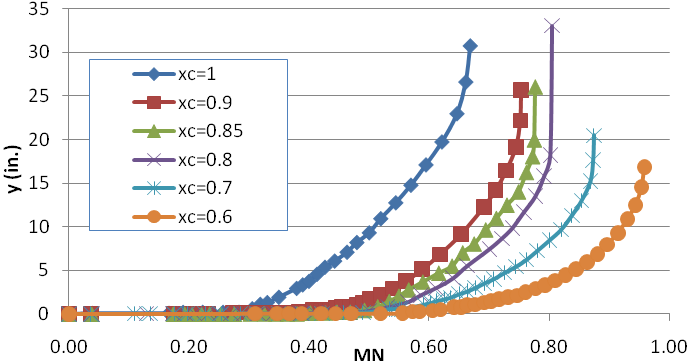
\includegraphics[width=120mm, height =70mm, clip=true]{Figure8_Boundary_Layers.png}
				\caption{Boundary layers profiles based on the Boeing HWB design and CFD analysis.  Plot of height above the airframe vs. axial Mach number. \cite{Fedler2011}}
				\label{Boundary_Layer_Profiles}
			\end{figure}
			%%
		\subsection{Integral Properties}
			\indent Based on this data, the boundary layer integral properties can be calculated along the airframe and the inviscid Mach number at the edge of the boundary layer can also be computed.  This data is shown in figure \ref{Integral_Properties} vs. the axial position along the aircraft centerline and shows that the properties grow as essentially the Reynolds length is increased.  The Mach number first increases along the suction side of the vehicle airfoil -- typically to a value that is transonic -- and then decreases on the aft end of the aircraft after about 60\% of the chord line due to the presence of the adverse static pressure gradient.
			%%
			\begin{figure}[htpb]
				\centering
				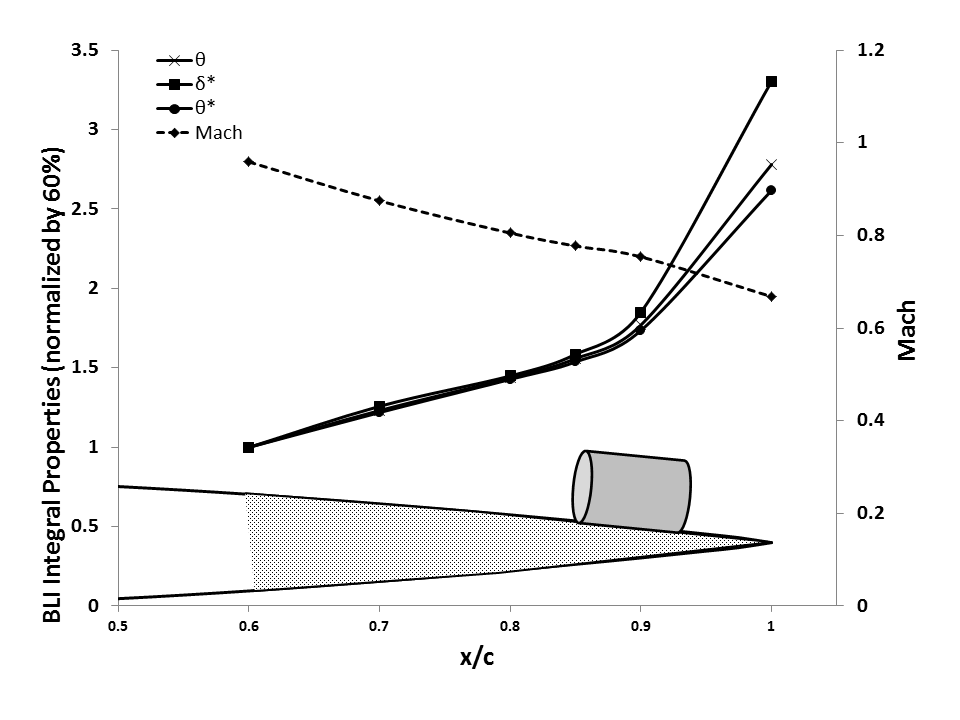
\includegraphics[width=120mm, height =70mm, clip=true]{Integral_Properties.png}
				\caption{Plot of Mach number, displacement, momentum, and kinetic energy defects vs. the axial length along the HWB centerline based on the Boeing CFD data.}
				\label{Integral_Properties}
			\end{figure}
			%%
			Analyzing figure \ref{Integral_Properties} and the equations for the power balance of the aircraft, it is clear that the BLI benefit terms in the power balance equation, as well as in the propulsive efficiency equation are increased as the engine is moved farther aft, since the momentum and kinetic energy defects are increased as the length along the aircraft is increased.  It is also worth noting that the engines placed outboard of this position may be subject to a different pressure gradient, Reynolds length, and fundamentally different intake aerodynamics than the center line engine and will thus have differences in the installation BLI impacts on engine performance.  This has yet to be sufficiently addressed in the current literature.
			\indent Another important point to be made is that for each flight condition, the angle of attack of the aircraft (typically set by lift and trim requirements) will have a strong impact on the flow entering the inlet.  It is thus necessary to map these boundary layer profiles as a function of this variable as well, which is not typically done.

		\subsection{Observations}
			\vspace{25pt}			
			\fbox{
			  \parbox{\textwidth}{
					Observation 1:  Existing system studies use either a simple 1-D boundary layer assumption or use tabular CFD data.  
					\vspace{5 mm}
				}
			}
	\section{BLI Inlet Modeling}
		Figure \ref{Inlet_Diagram} outlines the various regions of the flow field leading up to the fan face of the embedded engine.  The pre-entry boundary layer region was described in the previous section along with the models that are typically employed for conceptual level studies.  Additionally, there is the "pre-compression" region which is described by Plas in \cite{PlasThesis}.  This is the region in which the streamtube is affected by the presence of the engine and the flow is compressed into the inlet capture area.  Flow that is not ingested into the engine passes over the external cowl region which may typically induce some drag due to wall pressure or shock wave generation.  
			%%
			\begin{figure}[htpb]
			\centering
			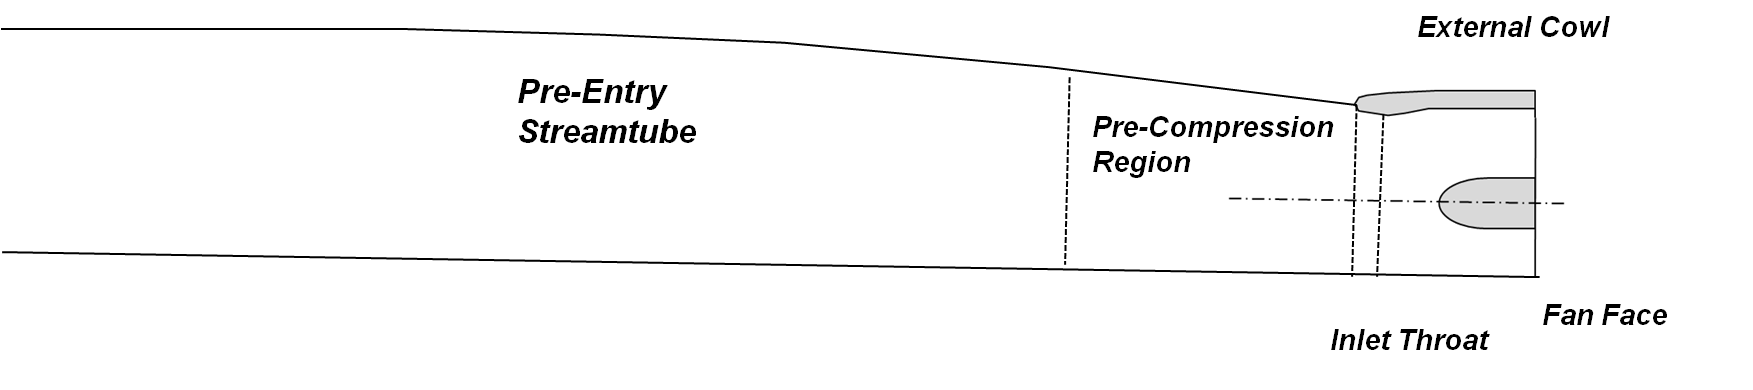
\includegraphics[width=160mm, height =45mm, clip=true]{Inlet_Diagram.png}
			\caption{Notional picture of the regions of the flow field before the fan face.}
			\label{Inlet_Diagram}
			\end{figure}
			%%
		 Inside the inlet, the Mach number decreases as the flow is diffused inside the inlet until it reaches the fan face.  The fan face Mach number is typically a function of the fan design specific flow capability. 
		
		\subsection{Pre-compression region}
			\indent Most of the system studies ignore the effect of the pre-compression region.  This includes \cite{Felder2011} \cite{Hardin2012}.  Plas \cite{PlasThesis} included a model of the pre-compression region using the integral boundary layer theory and modeling the static pressure distribution as an exponential and linear distribution within the region.  This approach yields a physics-based method for determining the evolution of the boundary layer properties and thicknesses within the pre-compression region.  

		\subsection{Inlet Sizing}
			With the presence of the boundary layer, the mass flow entering the inlet can be described in terms of the displacement thickness as follows:
			\begin{equation}
				\frac{\dot{m}}{\rho_eu_e} = \Big(A - b\delta^*\Big)
            \end{equation}%
			Here b is the width of the inlet assuming a constant width over the height of the boundary layer.  If the displacement thickness is known along with the inlet capture area geometry, then the required capture height of the stream tube prior to pre-compression can be calculated to satisfy the mass flow demand of the engine.  This was the approach used by Plas \cite{PlasThesis} to size the inlet capture area.  Other authors including \cite{Felder2012} have simply ignored the pre-compression region and used the boundary layer profiles from the CFD data for the purpose of direct integration to determine the necessary capture height.
			
			With the capture height calculation, one can mass average the total pressures and temperatures from the wall to the capture height to determine an average recovery.  Felder showed representative curves of mass-averaged total properties vs. capture height which are reproduced in figure \ref{Total_Properties}.  This data is again based upon the Boeing HWB design CFD analysis.
			%%
			\begin{figure}[htpb]
				\centering
				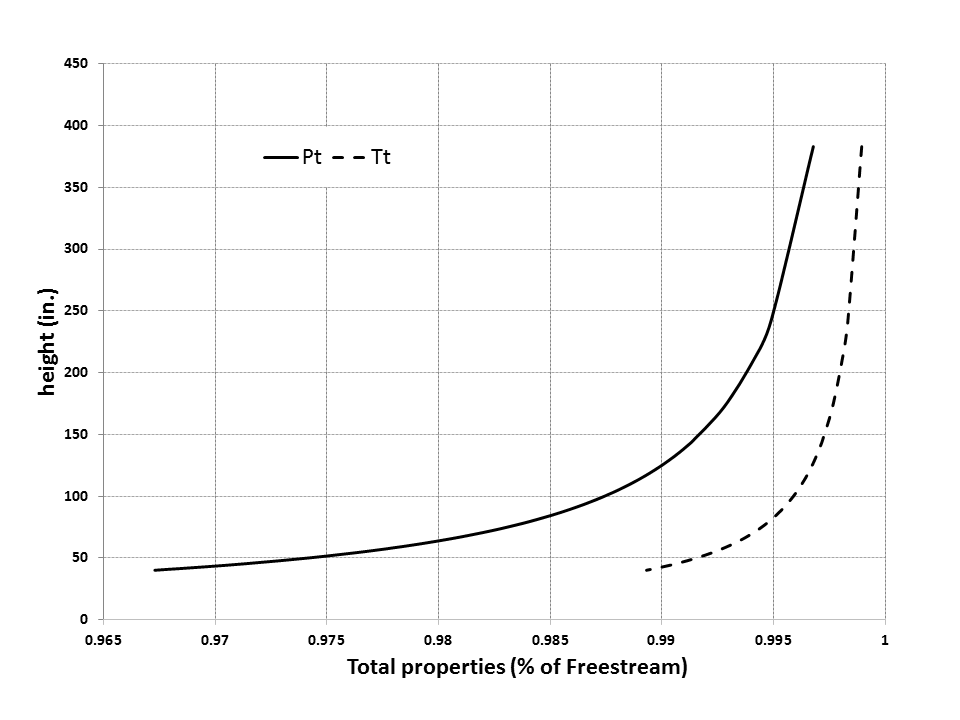
\includegraphics[width=130mm, height =100mm, clip=true, trim = 5mm 0mm 0mm 0mm]{Total_Properties.png}
				\vspace{-25pt}
				\caption{Mass averaged total pressure and temperature prior to the pre-compression region for the Boeing HWB design.}
				\label{Total_Properties}
			\end{figure}
			%%
		\subsection{Inlet Duct Recovery}
			Finally, the last component of the aerodynamic analysis prior to the fan face is the performance of the inlet duct.  The necessary output of this analysis depends upon the fidelity of the fan model used.  If the fan model requires more detailed fan face profiles, then a higher fidelity analysis must be used.  If the fan model requires only a characterization of the "dirty" or distorted region, then a simple 1-D type analysis might suffice, such as the integral boundary layer method \cite{PlasThesis}.  By far the most common approach, however, is the use of a simple inlet recovery parameter or inlet efficiency as is used in standard cycle analysis techniques.  This means that the BLI losses are essentially passed as a lower mass averaged pressure recovery to the standard fan analysis.  This approach is used in \cite{Felder2011} \cite{Sato2011} \cite{Hardin2012} \cite{Nickol2009}  with various values assumed for the pressure loss, which tends to have a significant impact on BLI performance.

	\section{Fan Modeling}
		\indent At the conceptual, system study level, the fan modeling approach taken is typically a simple efficiency hit.  This approach was used in \cite{Felder2011} \cite{Sato2011} \cite{Hardin2012} \cite{Nickol2009}  .  Although simple, it does provide a basic parametric way to understand the impact of the fan performance relative to the BLI propulsive efficiency benefits to understand technology targets for a BLI fan design.  Table \ref{Fan_Efficiency_Assumptions} shows the differences in assumptions used for the fan efficiency for some of the important system studies mentioned earlier.  It is common to assume that the efficiency penalty will be small, however recent work conducted by Pratt and Whitney \cite{Florea2013} shows that there is a likely efficiency penalty relative to a clean fan on the order of 0-1.5\%.  

		\begin{table}[ht]
			\caption{Fan efficiency assumption used for several system studies.}
			\renewcommand{\arraystretch}{1.5}% Spread rows out...
			\vspace{5pt}
			\centering
			\begin{tabular}{ >{\centering}P{3cm} |  >{\centering \arraybackslash}P{3cm} }
				\hline
				\bf{Reference} & \bf{$\eta$} duct \\
				\hline
				Dagget, 2003 & 0\% \\ 
				Kawai, 2006 & 0\%  \\
				Nickols, 2009 & 0\% \\
				Felder, 2011 & 1\% \\
				Hardin, 2012 & 0-8\% \\	
				\hline \hline			
			\end{tabular}
			\label{Fan_Efficiency_Assumptions}
		\end{table}

		As discussed previously, Plas \cite{Plas2007} conducted a study on 3 different levels of modeling fidelity for a ducted fan.  For brevity, the details of each model will not be discussed here, but rather some of the key conclusions from the study will be summarized and some observations will be made that are relevant for the current work.

		\subsection{Parallel Compressor Model}
			The basics of the parallel compressor model is to model the fan component as separate compressors with different total pressure, axial velocity, and mass flow but with the same speed and characteristic line (PR vs. corrected mass flow).  This model is useful because it creates a coupling between the nature of the distorted flow field (i.e. the magnitude of the $P_t$ deficit), the fan design via the characteristic, and the final efficiency and pressure ratio.  Figure \ref{PC_Figure} shows a simple illustration of the model on a fan map of PR vs. corrected mass flow.  
				%%
				\begin{figure}[htpb]
				\centering
				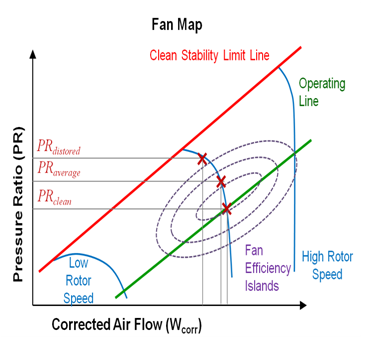
\includegraphics[width=90mm, height =60mm, clip=true, trim = 0mm 0mm 0mm 0mm]{PC_Figure.png}
				\caption{Illustration of the parallel compressor model on a notional fan map.}
				\label{PC_Figure}
				\end{figure}
				%%
			
			\indent The parallel compressor model used by Plas is essentially the simplest possible model because it employs a "2-segment" approach, with one dirty and one clean sector.  It is possible to include more sectors should the flow coming into the fan be proven to be more complex \cite{Greitzer1993}.  The parallel compressor model has been successfully used for performance prediction in the gas turbine industry and can also be used for operability prediction in certain cases.  Recent work has shown it's effectiveness for different types of inlet distortion in comparison to experimental rig data \cite{Cousins2011}.

		\subsection{Higher Fidelity Models}
			\indent Plas additionally employed two other higher fidelity models:  an integral boundary layer method and a 3-D body force model.  Both models showed differences from the PC approach ranging from 10-40\%, and more importantly, these approaches show the importance of the distortion attenuation and nozzle losses in determining the performance of the unducted propulsor.  This study shows that the attenuation must be modeled in some way and viewed parametrically, and also that the fidelity of simpler models can have significant impact on the viability of a BLI system.  The difficulty with the 3-D models is that it requires computationally expensive high-fidelity physics calculations, meaning that it is difficult to make the approach parametric for large design space explorations.  Additionally, a designer would ideally like to have a map for off-design performance calculations, so for each design a separate 3-D map would need to be created.  This makes the 3-D approaches somewhat less appealing in the context of conceptual design.  

		\subsection{Fan Distortion}
			As shown by the parallel compressor model, the performance of the fan can be impacted by the presence of inlet distortion.  However, perhaps more significantly is the impact on the fan stall margin.  Figure \ref{PC_Figure} shows that the dirty sector of the distortion is closer to the stall margin because the PR is more and the mass flow less in that region.  SAE ARP1420 \cite{ARP1420} provides parameters that can describe a total pressure distortion for an inlet aerodynamic interface plane (AIP).  Figure \ref{Circumferential_Distortion} illustrates a circumferential variation in the total pressure at a particular radial location for a single-per-rev type distortion (one continuous dirty sector).
				%%
				\begin{figure}[htpb]
				\centering
				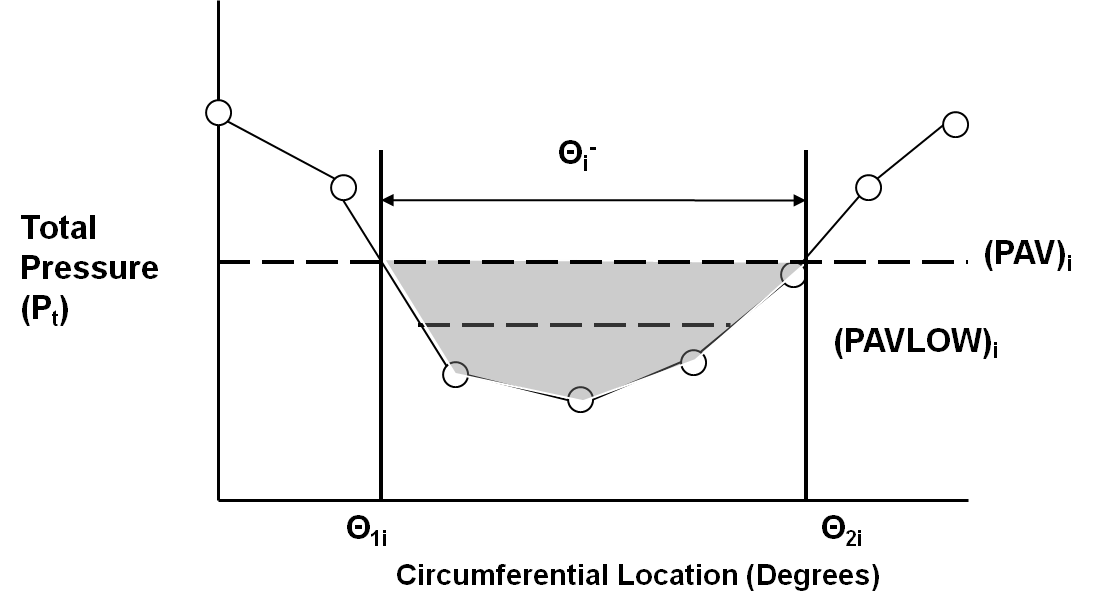
\includegraphics[width=110mm, height =70mm, clip=true, trim = 0mm 0mm 0mm 0mm]{Circumferential_Distortion.png}
				\caption{Typical circumeferential distortion distribution for a single-per-rev type distortion profile at the $i_{th}$ radial ring.}
				\label{Circumferential_Distortion}
				\end{figure}
				%%
			The circumferential distortion prescribed by ARP1420 guidelines is given by equation \ref{Circum_Descriptor}, where the terms in the equations are defined by equations \ref{Paverage} and \ref{PaverageLow}.
			\begin{equation}
				\Big(\frac{\Delta PC}{P}\Big)_i = \Big(\frac{PAV-PAVLOW}{PAV}\Big)_i
				\label{Circum_Descriptor}
			\end{equation}%

			\begin{equation}
				PAV_i = \frac{1}{360} \int_0^{360}{P(\theta)_i d\theta}
				\label{Paverage}
			\end{equation}%

			\begin{equation}PAVLOW_i = \frac{1}
			                                                 {\theta_i^-}\int_{\theta_{1i}}^{\theta_{2i}}{P(\theta)_i d\theta}
			\label{PaverageLow}\end{equation}%
			
			Finally, the radial distortion prescribed by ARP1420 is shown in equation \ref{Radial_Descriptor}, where PFAV is given by equation \ref{PFAV} and is the averaged over the i radial rings.
			\begin{equation}
				\Big(\frac{\Delta PR}
					    {P}\Big)_i = \frac{PFAV-PAV_i}
								{PFAV}
			\label{Radial_Descriptor}\end{equation}%
			
			\begin{equation}
				PFAV = \frac{1}
					         {N} \sum\limits_{i=1}^{N} PAV_i
			\label{PFAV}\end{equation}%
			
			Analyzing the above equations, one point seems salient, namely that the lower the average pressure, the higher the circumferential and radial distortion descriptors.  This means that if the stall margin reduction is correlated with the descriptor, as is typically done, then lowering the heights of the inlet using smaller inlet heights and more engines should tend to move the fan closer to the stall line.  Thus, there may be, depending on the fan characteristic and quality of the fan inlet flow, a point where smaller engines are simply limited by the operability constraint. 
			
			To date there have been no significant efforts to incorporate the operability concerns into the boundary layer ingestion modeling approaches at the conceptual level.  Perhaps the closest attempt to do so was done by Rodriguez for the case of the 3 engine BWB configuration.  His approach was to simply use distortion descriptors as a constraint on the inlet design, so that the optimization would maintain sufficiently low distortion while maximizing efficiency.  This may, in fact, prove useful in the preliminary design phase of the inlet, but remains difficult at the conceptual level when the general propulsion system layout has yet to be determined and is perhaps even more difficult for engine designers who may need to make decision before such high fidelity modeling is available.
			
			\vspace{25pt}			
			\fbox{
				\parbox{\textwidth}{
					Observation 2:  None of the system studies to date have considered operability within the context of engine sizing for boundary layer ingesting engines.
				}
			}
				 
\subsection{Gap Analysis}

\section{Towards A Solution}
	\subsection{Multi-Design Point Methodology Background}		
		\indent The preceeding section established that although cruise is the primary condition where the performance of the engine is most consequential in terms of fuel burn, that there are several other "off-design" conditions where the engine thrust capability must be sufficient and might therefore be candidates for inclusion into the engine cycle selection process.  The traditional engine design process has been performed at a single design point to set the cycle.  Performance at other operating conditions is then evaluated in off-design analysis.  Though this standard approach provides a good basis for understanding the trends of gas turbine performance, it does not provide a practical approach for a designer to match an engine and performance requirements for a particular airframe.  
		
		\indent Schutte \cite{SchutteThesis} designed and analyzed a methodology called simultaneous "multi-point design", in which modern computational tools are used in an engine sizing process which simultaneously satisfies engine requirements and constraints at multiple flight conditions.  This is done by linking engine "On-Design" and "Off-Design" within a modified Newton-Raphson solver to satisfy the thrust constraints at all conditions.  The process is necessary because it allows the formation of an engine cycle design space where each candidate cycle design is inherently feasible so long as the technology assumptions are physically achievable.  This eliminates needless manual iteration between the single point engine "On-Design" solutions and other off-design solutions.  The MDP concept is shown graphically in figure \ref{MDP_System_of_Equations}.  The design points are linked via the simultaneous solution of a system of equations.		
		%%
		\begin{figure}[htpb]
			\centering
			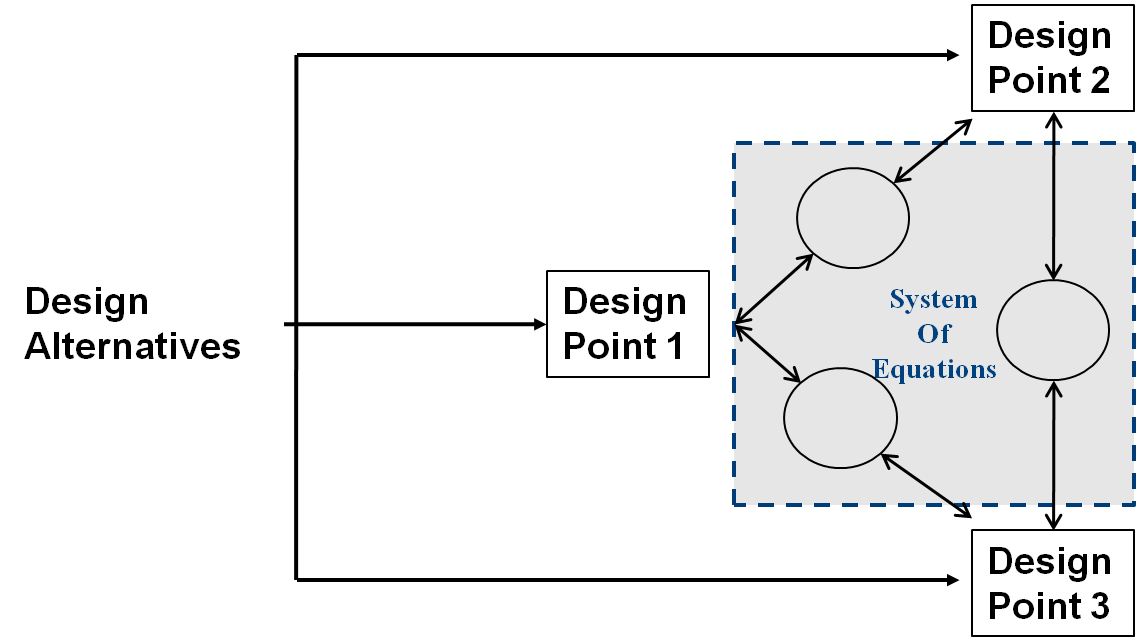
\includegraphics[width=110mm, height =70mm, clip=true, trim = 0mm 0mm 0mm 0mm]{MDP_System_of_Equations.png}
			\caption{Simultaneous multi-design point cycle analysis equation setup \cite{SchutteThesis}}
			\label{MDP_System_of_Equations}
		\end{figure}
		%%
		The MDP process is broken down into 3 parts:  the requirements and technology definition phase; the MDP setup phase; and the MDP execution phase.  The data flow chart for this process is shown in figure \ref{MDP_Methodology}.
		\begin{figure}[htp]
			\centering
			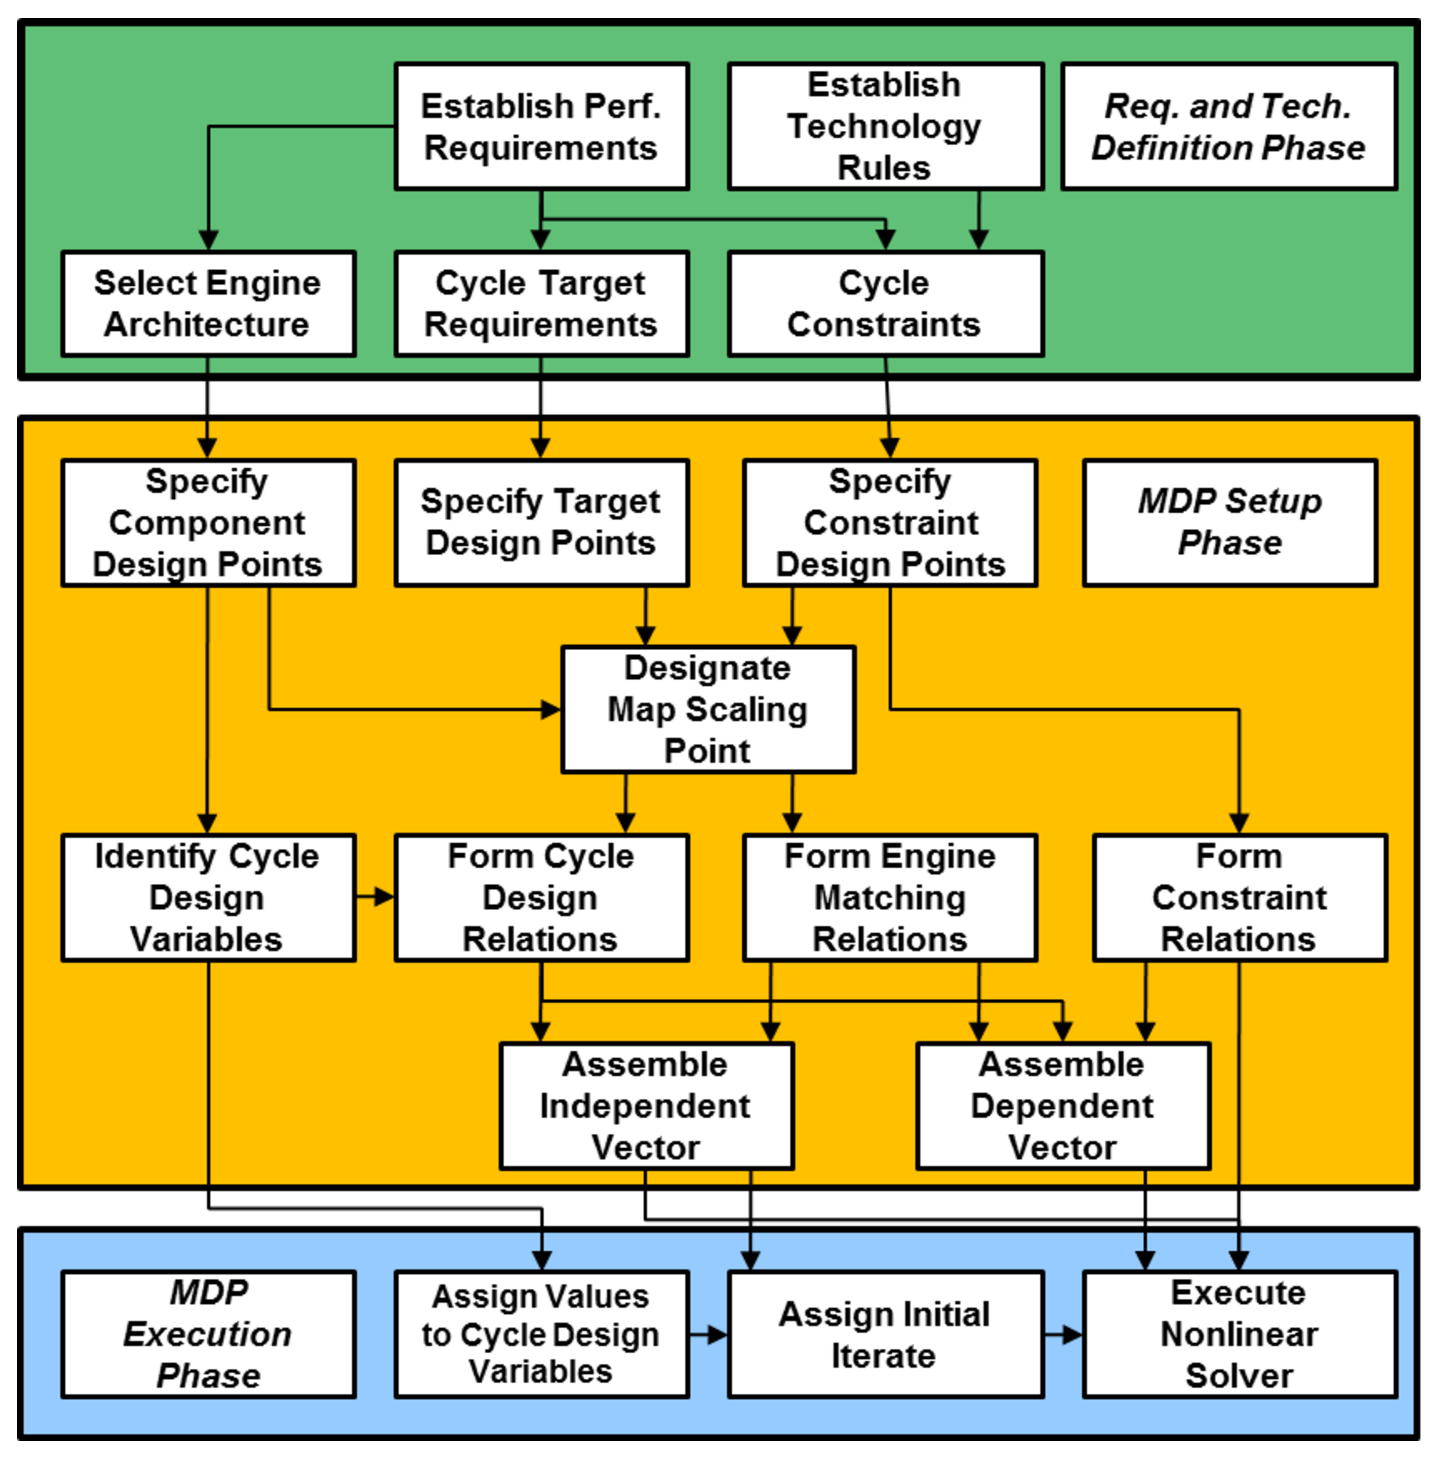
\includegraphics[scale = 0.4]{MDP_Methodology.eps}
			\caption{MDP Methodology Data Flow Chart}
			\label{MDP_Methodology}
		\end{figure}		
		The requirements and technology definition phase is general enough to handle any arbitrary operating (design) condition, which is one of the fundamental gaps in the current BLI literature.  Furthermore, it is also able to impose certain flight conditions as a cycle "constraint" condition.  If a condition is a critical distortion pinch point in the flight envelope, it could be used as a cycle constraint condition within an MDP analysis.  Technology rules for how the distortion is handled or how much is allowable can then be specified to affect the operating point of the engine to move sufficiently away from the fan stall line.  Impacts of the distortion related technology rules on the performance of the engine at the other sizing conditions would then be automatically known to the designer.  For these reasons, the MDP design process will be the starting point for moving towards a new paradigm for BLI cycle analysis.
		
	\subsection{Short-Comings of the MDP Process for BLI}  
		Though the MDP process is an appealing starting point for moving towards a proper BLI propulsion system sizing approach, there are a few areas where doing MDP alone is not sufficient for filling in the gaps described above.
		
		\begin{itemize}
			\item{MDP does not describe how the installation effects of BLI are to be modeled or mapped across the different flight conditions.  It merely assumes that the designer has constructed a proper mapping of the installation effects a-priori.  The same goes for the modeling of distortion and how that is achieved.}
			\item{MDP does not deal with the problem of distributed architectures, in which the inlet conditions are different across a propulsor array.  Rather, it is designed specifically for typical gas turbine arrangement on current tube and wing aircraft.}
			\item{The designer using an MDP may not know the flight conditions which are most critical for new concepts such as BLI, where installation effects could have a significant impact on the location of the critical sizing and operability conditions in the flight envelope.}
		\end{itemize}
		
	\subsection{Research Objective}
		From the above considerations, a research objective has been formulated and is stated as follows:				
		
		\vspace{1pt}
		\vspace{5mm}
		\noindent{
			\fbox{
				\parbox{\textwidth}{
					\textbf{Research Objective}:  Develop a methodology for conceptual system level sizing and analysis of BLI propulsion systems which can quantify BLI performance impacts over a range of system operating conditions, determine the impact of architecture and cycle choices on performance and operability, determine critical design conditions for the system, and allow for simultaneous satisfaction of system requirements and constraints at multiple design conditions.
				}
			}
		}